\section{TINJAUAN PUSTAKA}

% Ubah konten-konten berikut sesuai dengan isi dari tinjauan pustaka

%UU LALU LINTAS DAN ANGKUTAN JALAN
\subsection{UU Lalu Lintas dan Angkutan jalan}
\label{sec:uulalulintas}
UU Lalu lintas dan Angkutan Jalan merupakan undang-undang berisi untuk mengatur
mengenai penyelenggara lalu lintas dan angkutan jalan, seperti pengaturan, pengendalian, perencanaan serta
pengawasan. Undang-undang tersebut diterbitkan pada tahun 2009 oleh Dewan Perwakilan Rakyat Republik Indonesia (DPR RI) yang mempunyai
tujuan seperti yang tertuang pada pasal 3 UU. No. 22 tahun 2009 tentang lalu lintas dan angkutan umum yang berisi sebagai berikut: \citep{angkutan-jalan}
\begin{enumerate}[nolistsep]
  \item \emph{Terwujudnya pelayanan Lalu Lintas dan Angkutan Jalan yang aman, selamat, tertib, lancar, dan terpadu dengan moda angkutan lain untuk mendorong perekonomian nasional, memajukan kesejahteraan umum, memperkukuh persatuan dan kesatuan bangsa, serta mampu menjunjung tinggi martabat bangsa.}
  \item \emph{Terwujudnya etika berlalu lintas dan budaya bangsa.}
  \item \emph{Terwujudnya penegakan hukum dan kepastian hukum bagi masyarakat.}
\end{enumerate}

%SEPEDA MOTOR
\subsubsection{Sepeda Motor}
\label{subsec:sepedamotor}
Definisi sepeda motor tertulis pada pasal 1 ayat (20) UU. No.22/2009 Tentang Lalu
Lintas dan Angkutan Umum yang berbunyi: \emph{"Sepeda Motor adalah Kendaraan Bermotor
beroda dua dengan atau tanpa rumah-rumah dan dengan atau tanpa kereta samping atau
Kendaraan Bermotor beroda tiga tanpa rumah-rumah."}

%ATURAN PENGGUNAAN HELM
\subsubsection{Aturan Pengunaan Helm}
\label{subsec:helm}
Peraturan penggunaan helm bagi pengendara sepeda motor diatur pada pasal 57 ayat (1) dan ayat (2) UU. No. 22 tahun 2009
Tentang Lalu Lintas dan Angkutan Jalan yang berisi:
\begin{enumerate}[nolistsep]
  \item \emph{Setiap Kendaraan Bermotor yang dioperasikan di Jalan
  wajib dilengkapi dengan perlengkapan Kendaraan
  Bermotor.} 
  \item \emph{Perlengkapan sebagaimana dimaksud pada ayat (1) bagi
  Sepeda Motor berupa helm standar nasional Indonesia.}
\end{enumerate}

Lalu pada pasal 291 UU. No.22/2009 dijelaskan juga sanksi bila melanggar peraturan tidak menggunakan
helm saat mengendarai sepeda motor seperti berikut:
\begin{enumerate}
  \item \emph{Setiap orang yang mengemudikan Sepeda Motor tidak
  mengenakan helm standar nasional Indonesia
  sebagaimana dimaksud dalam Pasal 106 ayat (8)
  dipidana dengan pidana kurungan paling lama 1 (satu)
  bulan atau denda paling banyak Rp250.000,00 (dua
  ratus lima puluh ribu rupiah).} 
  \item \emph{Setiap orang yang mengemudikan Sepeda Motor yang
  membiarkan penumpangnya tidak mengenakan helm
  sebagaimana dimaksud dalam Pasal 106 ayat (8)
  dipidana dengan pidana kurungan paling lama 1 (satu)
  bulan atau denda paling banyak Rp250.000,00 (dua
  ratus lima puluh ribu rupiah).}
\end{enumerate}
 

% Contoh input gambar

% Per Teori Penunjang dibuat section baru
% MACHINE LEARNING
\subsection{\emph{Machine Learning}}
\label{sec:machinelearning}

\emph{Machine Learning} merupakan sebuah cabang ilmu bagian dari kecerdasan buatan \emph{(artificial intelligence)}
dengan input pemrograman untuk memungkinkan komputer mempelajari sebuah perilaku dan meningkatkan
pemahamannya melalui pengalaman secara otomatis \citep{machinelearning}. \emph{Machine Learning} memiliki fokus pada pengembangan sistem yang mampu belajar
sendiri untuk memutuskan sesuatu tanpa harus berulang kali diprogram oleh manusia. Masalah ini
membuat mesin mampu tidak hanya membuat keputusan, tetapi juga
beradaptasi dengan perubahan yang terjadi. Pembelajaran mesin berfungsi saat data tersedia
sebagai masukan untuk analisis kumpulan data yang besar (big data) sehingga
menemukan pola tertentu. Data adalah bahan masukan yang akan digunakan untuk melakukan
pembelajaran (pelatihan) agar mesin dapat menghasilkan analisis yang benar. Di
pembelajaran mesin dikenal sebagai pelatihan data dan pengujian data, data pelatihan untuk melatih algoritma
dalam pembelajaran mesin dan pengujian data untuk menentukan kinerja algoritma di
machine learning yang sudah dilatih adalah ketika menemukan data baru yang belum pernah ada
diberikan dalam data pelatihan \citep{machinelearning2}

%SUPERVISED LEARNING
\subsubsection{\emph{Supervised Learning}}
\label{subsec:supervisedlearning}

\emph{Supervised learning} merupakan sebuah pendekatan \emph{machine learning} dalam menciptakan
\emph{artificial intelligence} yang dimana algoritma komputer dilatih menggunakan data \emph{input} yang telah
diberikan label untuk hasil \emph{output} tertentu. Model dilatih hingga dapat mendeteksi pola dan hubungan yang menjadi dasar
anatara data \emph{input} dan \emph{output}, sehingga memungkinkannya hasil pelabelan yang akurat saat disajikan dengan data yang belum
pernah diberi label.

%UNSUPERVISED LEARNING
\subsubsection{\emph{Unsupervised Learning}}
\label{subsec:unspervisedlearning}

\emph{Unsupervised learning} merupakan sebuah pendekatan \emph{machine learning} menggunakan informasi yang tidak diklasifikasikan atau diberi label seperti
\emph{supervised learning}. Algoritma ini memungkinkan \emph{artificial intelligence} untuk bertindak sendiri berdasarkan informasi tanpa bantuan. Pada \emph{unsupervised learning} tugas dari
\emph{artificial intelligence} adalah mengelompokkan informasi yang tidak disortir berdasarkan
persamaannya, pola, serta perbedaan tanpa ada pelatihan data sebelumnya.
%REINFORCEMENT LEARNING
\subsubsection{\emph{Reinforcement Learning}}
\label{subsec:reinforcementlearning}

\emph{Reinforcement learning} merupakan sebuah pendekatan \emph{machine learning} untuk membuat urutan keputusan. Dalam pendekatan ini, mesin belajar untuk mencapai
tujuan dalam lingkungan yang tidak pasti dan berpotensi kompleks. \emph{Reinforcement learning} mempelajari keadaan sekitar seperti layaknya sebuah permainan, komputer menggunakan metode
\emph{trial and error} dalam menemukan solusi dari sebuah masalah. Untuk membuat mesin berjalan seperti yang \emph{programmer} inginkan, ditetapkan sebuah \emph{reward} dan \emph{penalties} dalam tindakan
mesin tersebut, tujuannya adalah mendapatkan \emph{rewards} yang akan dikembalikan kepada \emph{agent}. Meskipun \emph{designer} menetapkan kebijakan \emph{rewards}, mesin tidak diberikan petunjuk atau saran
kepada model bagaimana cara menyelesaikan permainan tersebut. Terserah model untuk mengetahui bagaimana melakukan tugas untuk memaksimalkan \emph{rewards}, mulai dari uji coba
yang benar-benar acak dan diakhiri dengan teknik yang canggih. Dengan memanfaatkan kekuatan pencarian dan banyak percobaan, \emph{reinforcement learning} pada saat ini adalah sebuah solusi 
yang paling efektif untuk memberikan saran dalam kreativitas mesin.

%DEEP LEARNING
\subsection{\emph{Deep Learning}}
\label{sec:deeplearning}

\emph{Deep learning} merupakan bagian dari \emph{machine learning} yang memungkinkan komputasi yang terdiri dari beberapa
lapisan pemrosesan untuk mempelajari representasi dara menggunakan berbagai tingkat abstraksi. \emph{Deep learning} memungkinkan untuk menemukan
struktur rumit dalam kompulan data besar dengan menggunakan algoritma \emph{backpropagation} untuk menunjukkan bagaimana mesin harus mengubah
parameter internal yang digunakan untuk menghitung representasi di setiap lapisan dari lapisan sebelumnya. \citep{lecun}

%NEURAL NETWORK
\subsubsection{\emph{Neural Network}}
\label{subsec:neuralnetwork}

\emph{Neural network} pertama kali dikenalkan oleh McCulloch dan Pitts pada tahun 1990 dalam percobaannya yaitu menemukan representasi
matematis dari pemrosesan informasi dalam sistem biologis. \emph{Neural networks} merupakan jaringan yang berasal dari \emph{node} (cabang), yang menirukan 
struktur neuron otak dari makhluk hidup. \emph{Node} menghitung jumlah nilai bobot dari masukan dan memprosesnya pada \emph{hidden layer} (lapisan tersembunyi), lalu 
mengeluarkan hasil dari fungsi pengaktifan dengan nilai bobot.

\emph{Neural networks} telah dikembangkan dari sebuah arsitektur sederhana menjadi struktur yang semakin
kompleks. Pada awalnya, \emph{neural networks} pertama kalinya memiliki arsitektur yang sangat sederhana yang terdiri dari lapisan \emph{input} dan \emph{output} atau dapat
disebut sebagai jaringan \emph{single-layer}. Ketika \emph{hidden layer} ditambahkan ke jaringan neuron \emph{single-layer}, maka akan menghasilkan
jaringan saraf \emph{multi-layer}. Oleh karena itu, jaringan saraf \emph{multi-layer} terdiri atas lapisan \emph{input}, \emph{hidden-layer}, dan lapisan \emph{output} seperti pada Gambar 2.1.
\begin{figure}[ht]
  \centering

  % Ubah dengan nama file gambar dan ukuran yang akan digunakan
  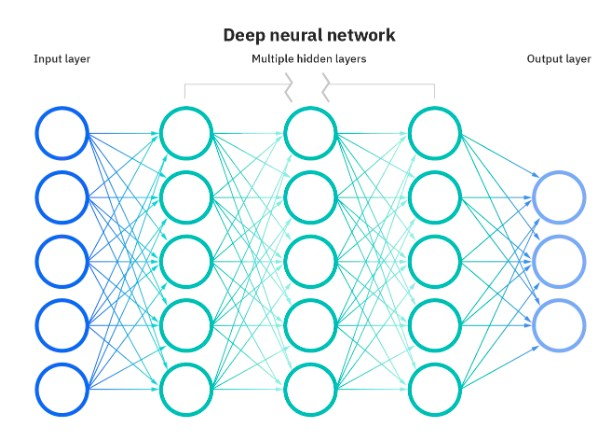
\includegraphics[scale=0.7]{gambar/neural-network.jpg}

  % Ubah dengan keterangan gambar yang diinginkan
  \caption{Struktur dari \emph{neural network}.}
  \label{fig:neural-network}
\end{figure}

Untuk mendapatkan neuron tujuan(y) maka nilai yang terdapat dari neuron(x) dikalkulasi dengan bobot(w) dan ditambahkan
dengan bias(b) lalu diaktivasi menggunakan fungsi(g) yang akan menentukan neuron selanjutnya(y) seperti persamaan 2.1 berikut.
\begin{equation}
  \label{eq:pers-neural-network}
  y = g (\sum_{i = 1}^{n}x_i w_i + b)
\end{equation}


\subsection{\emph{Convolutional Neural Network (CNN)}}
\label{sec:cnn}
\emph{Convolutional Neural Network} (CNN) merupakan cabang dari Multilayer Perceptron
(MLP) yang digunakan untuk mengolah data dua dimensi. CNN memiliki kedalaman
jaringan yang tinggi sehingga CNN termasuk dalam jenis Deep Neural Network. Perbedaan
CNN dengan MLP terdapat pada neuron dimana pada MLP setiap neuron hanya berukuran
satu dimensi, sedangkan CNN setiap neuronnya berukuran dua dimensi. Pada CNN, operasi
linier menggunakan operasi konvolusi. Bobot pada CNN berbentuk empat dimensi seperti pada Gambar 2.2. Persamaan 2.2 untuk dimensi
bobot pada CNN.
\begin{equation}
  neuron  Input \times neuron  Output \times tinggi \times lebar
\end{equation}

\begin{figure}[ht]
  \centering

  % Ubah dengan nama file gambar dan ukuran yang akan digunakan
  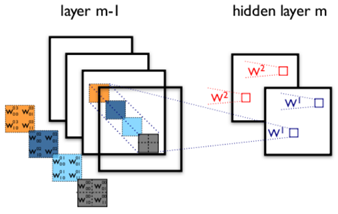
\includegraphics[scale=0.8]{gambar/proses konvolusi.png}

  % Ubah dengan keterangan gambar yang diinginkan
  \caption{Proses Konvolusi dari CNN.}
  \label{fig:convolutional-neural-network}
\end{figure}

\subsubsection{\emph{Convolutional Layer}}
\label{subsec:convolutional-layer}
\emph{Convolutional layer} merupakan proses utama dalam metode CNN yang bertugas menjalankan operasi konvolusi pada \emph{output} dari \emph{layer} sebelumnya. 
Konvolusi yaitu mengaplikasikan sebuah fungsi pada \emph{output} fungsi lainnya secara berulang-ulang. Seperti pada Gambar 2.3, konvolusi
mengaplikasikan kernel yang berwarna kuning pada citra yang terdapat pada semua \emph{offset}. Kotsk hijau secara keseluruhan adalah sebuah citra yang
akan dikonvolusi, kernel bergerak dari sudut kiri atas ke kanan bawah, sehingga hasi konvolusi dari citra tersebut dapat dilihat pada gambar bagian kanan.

\begin{figure}[ht]
  \centering

  % Ubah dengan nama file gambar dan ukuran yang akan digunakan
  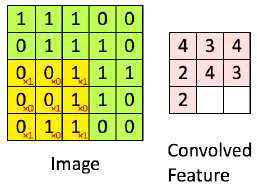
\includegraphics[scale=0.8]{gambar/konvolusi-cnn.jpg}

  % Ubah dengan keterangan gambar yang diinginkan
  \caption{Ilustrasi Proses Konvolusi dari CNN.}
  \label{fig:convolutional-neural-network}
\end{figure}

Tujuan dilakukannya konvolusi pada data citra adalah untuk mengekstraksi fitur dari citra \emph{input}. Konvolusi akan menghasilkan transformasi linier dari data input sesuai dengan
informasi spasial pada data. Bobot pada layer tersebut menspesifikasikan kernel konvolusi yang digunakan, sehingga kernel berkonvolusi dapat
dilatih bersamaan input pada CNN.

\subsubsection{\emph{Subsampling Layer}}
\label{subsec:subsampling-layer}

Subsampling Layer adalah proses mereduksi ukuran pada sebuah data citra. Tujuannya adalah untuk meningkatkan invariansi posisi dari fitur.
Dalam CNN, metode subsampling yang digunakan adalah \emph{max pooling}. Pada ilustrasi pada Gambar 2.4, \emph{Max pooling} membagi output
dari convolution layer menjadi beberapa grid kecil lalu mengambil
nilai maksimal dari setiap grid untuk menyusun matriks citra yang
telah direduksi. Grid yang berwarna merah, hijau, kuning dan biru merupakan kelompok grid yang akan dipilih nilai maksimumnya.
Sehingga hasil dari proses tersebut dapat dilihat pada kumpulan
grid disebelah kanannya. Proses tersebut memastikan fitur yang
didapatkan akan sama meskipun objek citra mengalami translasi
(pergeseran). Penggunaan pooling layer pada CNN hanya bertujuan untuk mereduksi ukuran citra sehingga dapat dengan mudah
digantikan dengan sebuah convolution layer dengan stride yang sama dengan pooling layer yang bersangkutan.

\begin{figure}[ht]
  \centering

  % Ubah dengan nama file gambar dan ukuran yang akan digunakan
  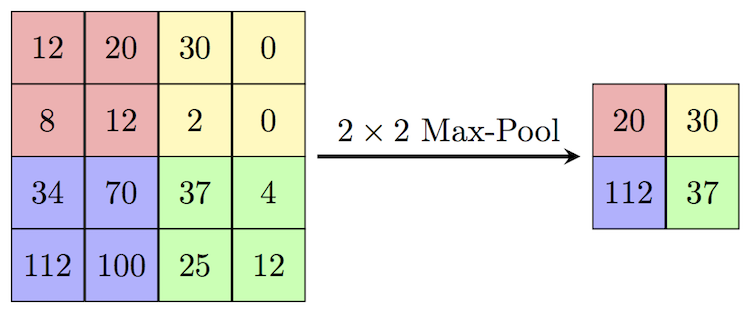
\includegraphics[scale=2]{gambar/MaxpoolSample.png}

  % Ubah dengan keterangan gambar yang diinginkan
  \caption{Ilustrasi Proses \emph{max pooling} dari CNN.}
  \label{fig:convolutional-neural-network}
\end{figure}


\subsubsection{\emph{Fully Connected Layer}}
\label{subsec:fullyconnectedlayer}

Fully-Connected Layer bertujuan untuk melakukan transformasi pada dimensi data agar data dapat diklasifikasikan secara linier. Setiap neuron pada convolution layer perlu ditransformasi menjadi data satu dimensi terlebih dahulu sebelum dapat dimasukkan
ke dalam sebuah fully connected layer. Karena hal tersebut menyebabkan data kehilangan informasi spasialnya dan tidak reversibel,
fully connected layer hanya dapat diimplementasikan diakhir jaringan. Convolution layer dengan ukuran kernel 1 × 1 melakukan fungsi
yang sama dengan sebuah fully connected layer namun dengan tetap
mempertahankan karakter spasial dari data.


\subsection{Visi Komputer}
\label{sec:viskom}

Visi Komputer adalah cabang Artificial Intelligent (AI) yang mencakup proses analisa
citra dan video. Visi komputer mengimplementasikan beberapa kemampuan visual manusia
yang diteruskan menuju otak seperti deteksi benda, pengenalan wajah dan mengenali
bahaya. Pada visi komputer, Deep Learning sering digunakan untuk pengenalan dan
deteksi objek. Proses Deep Learning pada visi komputer memanfaatkan piksel pada citra
untuk ekstrasi pola atau atribut dari citra yang ingin dideteksi. Akan tetapi, hal tersebut
mengakibatkan sistem komputasi menjadi lama karena pada suatu citra mengandung
ribuan piksel.

\subsection{\emph{Image Processing}}
\label{sec:image-Processing}

\emph{Image Processing} atau Pengolahan Citra adalah sebuah teknik
pemrosesan gambar dengan input berupa sebuah citra dua dimensi yang memiliki tujuan untuk menyempurnakan citra atau mendapatkan
informasi yang berguna untuk diolah menjadi beberapa keputusan. Dalam operasi pemrosesan citra, operasi yang sering dilakukan
dalam gambar \emph{grayscale}. Gambar \emph{grayscale} didapatkan dari pemrosesan gambar berwarna yang didekomposisi menjadi komponen
merah (R), hijau (G) dan biru (B) yang diproses secara independen
sebagai gambar \emph{grayscale}. \emph{Image Processing} terbagi menjadi dalam 3 tingkatan:

\begin{enumerate}
  \item \emph{Low-Level Image Processing} merupakan operasi sederhana dalam pengolahan gambar dimana input dan output berupa gambar. Contoh: contrast enchancement dan noise reduction.
  \item \emph{Mid-Level Image Processing} merupakan operasi pengolahan
  gambar yang melibatkan ekstrasi atribut dari gambar input.
  Contoh: \emph{contours}, \emph{edge} dan \emph{regions}.
  \item \emph{High-Level Image Processing} merupakan merupakan kategori
  yang melibatkan pemrosesan gambar kompleks yang terkait
  dengan analisis dan interpretasi konten dalam sebuah keadaan
  untuk pengambilan keputusan.
\end{enumerate}

\subsubsection{\emph{Digital Image}}
\label{subsec:digital-image}
\emph{Digital Image} merupakan fungsi dua dimensi f(x,y) yang merupakan proyeksi dari bentuk tiga dimensi kedalam bentuk dua dimensi dimana x dan y merupakan lokasi elemen gambar atau piksel yang berisikan nilai. Ketika nilai x,y dan intensitasnya berupa
diskrit, maka gambar tersebut dapat dikategorikan sebagai digital
image. Secara matematis, \emph{digital image} adalah representasi matriks
dari gambar dua dimensi menggunakan piksel. Setiap piksel diwakili oleh nilai numerik. Untuk gambar grayscale, hanya memiliki satu
nilai dengan kisaran antara 0-255.Pada Gambar 2.5, untuk gambar yang berwarna, memiliki tiga nilai yang mewakili merah (R),
hijau (G) dan biru (B) yang masing-masing memiliki kisaran nilai
yang sama antara 0-255. Jika suatu gambar hanya memiliki dua
intensitas, gambar tersebut dikenal sebagai \emph{binary image}.
\begin{figure}[ht]
  \centering
  % Ubah dengan nama file gambar dan ukuran yang akan digunakan
  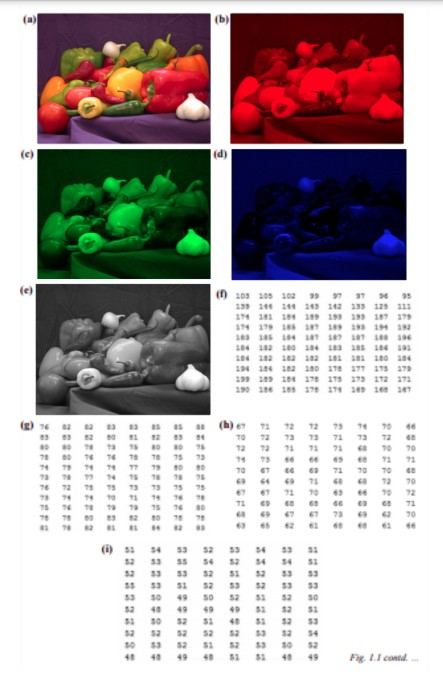
\includegraphics[scale=0.7]{gambar/digital-image-arch.jpg}
  % Ubah dengan keterangan gambar yang diinginkan
  \caption{: (a) Gambar berwarna, (b) Komponen merah dalam gambar berwarna, (c) Komponen hijau dalam gambar bewarna, (d) Komponen biru dalam gambar bewarna, (e) Gambar bewarna dikonversi dalam
  8-bit grayscale, (f) Matriks dari gambar (b), (g) Matriks dari gambar (c),
  (h) Matriks dari gambar (d), (i) Matriks dari gambar (e)}
  \label{fig:digital-image}
\end{figure}

\subsection{\emph{You Only Look Once} (YOLO)}
\label{sec:YOLO}
\emph{You Only Look Once} (YOLO) merupakan sistem deteksi yang
berbasis \emph{Convolutional Neural Network}. Pada Gambar 2.6, Dalam
arsitektur YOLO terdiri dari 24 convolutional layer yang berfungsi sebagai mendapatkan fitur dari citra. Kemudian diikuti dua connected layer yang berfungsi sebagai memprediksi probabilitas dan
koordinat, Seperti pada Gambar 2.7, terdapat tiga langkah deteksi objek menggunakan YOLO seperti berikut:
\begin{enumerate}
  \item Mengubah ukuran dimensi masukan citra menjadi 448 × 448.
  \item Menjalankan single convolutional network pada citra.
  \item Melakukan threshold pada hasil deteksi berdasarkan nilai confidence yang didapatkan oleh model.
\end{enumerate}

Pada proses pertama, YOLO mendeteksi objek menggunakan unified detection yang menyatukan antara komponen deteksi objek kedalam single neural network. Desain YOLO memungkinkan end-toend training dan real-time speed dengan mempertahankan rata-rata
presisi yang tinggi. Sistem pada YOLO membagi gambar masukan
kedalam grid S × S. Jika titik tengah dari sebuah objek terdapat
didalam salah satu sel, maka sel grid itu bertanggung jawab untuk
mendeteksi objek tersebut. Setiap sel kota memprediksi bounding
box B dan nilai confidence untuk setiap kotak. Nilai confidence
merepresentasikan keakuratan model bahwa terdapat objek dalam
bounding box tersebut. Setiap bounding box memiliki 5 parameter
prediksi yaitu x, y, w, h, seperti pada Gambar 2.8 dan confidence.
Koordinat (x,y) merupakan pusat dari kotak relatif ke gambar dan
confidence merupakan Intersection over Union (IoU) antara predicted box dengan ground-truth box. Setiap sel grid memprediksi
probabilitas kelas C. Setiap sel grid memprediksi nilai probabilitas
pada kelas C. Probabilitas tersebut dikondisikan berdasarkan sel
grid yang memuat objek. Sehingga hanya terdapat satu kelas probabilitas yang terdeteksi disetiap sel grid tanpa memperhitungkan
jumlah bounding box B. Saat deteksi, probabilitas kelas dikalikan
nilai confidence sesuai persamaan 2.3 atau disederhanakan menjadi seperti persamaan 2.4 \citep{yolo}.

\begin{equation}
  Pr(Class_i | Object) \times Pr(Object) \times truthIOUpred
\end{equation}
\begin{equation}
  Pr(Class_i)\times truthIOUpred
\end{equation}
\begin{figure}[ht]
  \centering
  % Ubah dengan nama file gambar dan ukuran yang akan digunakan
  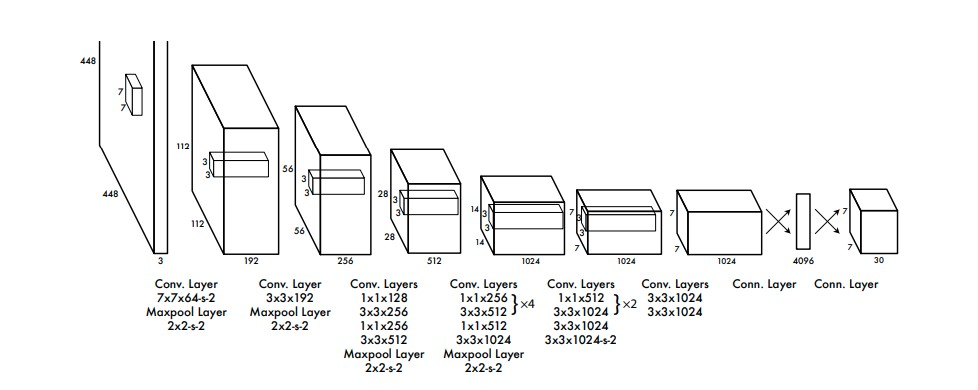
\includegraphics[scale=0.6]{gambar/arch_yolo.jpg}
  % Ubah dengan keterangan gambar yang diinginkan
  \caption{Arsitektur dari YOLO}
  \label{fig:arch-yolo}
\end{figure}
\begin{figure}[ht]
  \centering
  % Ubah dengan nama file gambar dan ukuran yang akan digunakan
  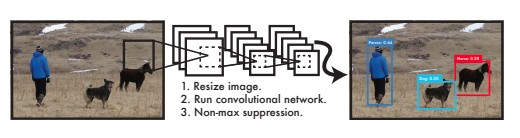
\includegraphics[scale=0.8]{gambar/sistem-deteksi-yolo.jpg}
  % Ubah dengan keterangan gambar yang diinginkan
  \caption{Sistem deteksi pada YOLO}
  \label{fig:sistem-deteksi-yolo}
\end{figure}

Dari persamaan tersebut, didapatkan nilai confidence dari kelas spesifik. Nilai ini merepresentasikan probabilitas kelas yang muncul didalam kotak dan seberapa baik kotak yang diprediksi akurat dengan
objek. Seperti pada ilustrasi pada Gambar 2.9, YOLO mendeteksi
model sebagai regresi. Hal ini membagi gambar menjadi grid dan
secara bersamaan memprediksi bounding box dan confidence pada
bounding box tersebut dan kelas probabilitas.

Pada YOLOv1, \emph{backbone} dari \emph{feature extraction} Darknet-19 memiliki kesulitan dalam mendeteksi objek kecil, sehingga
pada YOLOv3, \emph{backbone} tersebut diubah menggunakan Darknet-53 untuk menyelesaikan masalah tersebut. Dalam pengerjaannya, metode baru seperti \emph{Residual Block}, \emph{skip-connection}, dan \emph{up-sampling}, yang dimana secara signifikan
meningkatkan akurasi dari algoritma tersebut. YOLOv5 merupakan versi terbaru dari YOLO, yang dimana YOLOv5 ini
adalah versi ringan dari YOLO sebelumnya, pada YOLOv5 lebih mengoptimalkan penggunaan \emph{framework} PyTorch daripada menggunakan Darknet. Tabel perbandingan dari YOLOv3 dan YOLOv5 dapat dilihat pada Tabel 2.1 berikut:
\begin{table}
  \caption{Tabel Perbandingan YOLOv3 dan YOLOv5}
  \centering
  \begin{tabular}{|p{4cm}|p{4cm}|p{4cm}|} 
  \cline{2-3}
  \multicolumn{1}{l|}{}              & \textbf{YOLOv3}               & \textbf{YOLOv5}                                         \\ 
  \hline
  Tipe \textit{Neural Network}       & \textit{Fully Convolution}    & \textit{Fully Convolution}                              \\ 
  \hline
  \textit{Backbone Feature Extractor} & Darknet-53                    & CSPDarknet53                                            \\ 
  \hline
  \textit{Loss Function}             & \textit{Binary Cross Entropy} & \textit{Binary Cross Entropy and Logits loss Function}  \\ 
  \hline
  \textit{Neck}                      & FPN                           & PANet                                                   \\ 
  \hline
  \textit{Head}                      & YOLO layer                    & YOLO layer                                              \\
  \hline
  \end{tabular}
\end{table}


\begin{figure}[ht]
  \centering
  % Ubah dengan nama file gambar dan ukuran yang akan digunakan
  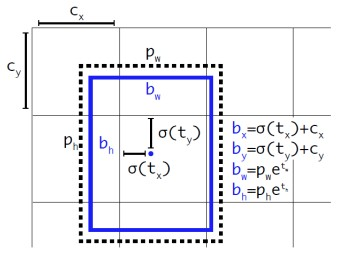
\includegraphics[scale=0.7]{gambar/bounding-box.jpg}
  % Ubah dengan keterangan gambar yang diinginkan
  \caption{Bounding box pada YOLO}
  \label{fig:bounding-box}
\end{figure}

\begin{figure}[ht]
  \centering
  % Ubah dengan nama file gambar dan ukuran yang akan digunakan
  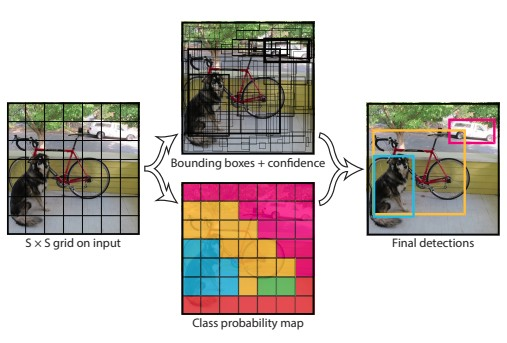
\includegraphics[scale=0.7]{gambar/proses-deteksi-yolo.jpg}
  % Ubah dengan keterangan gambar yang diinginkan
  \caption{Proses deteksi pada YOLO}
  \label{fig:deteksiyolo}
\end{figure}

\subsubsection{Arsitektur YOLOv3}
\label{subsec:arsitektur-yolov3}
Pada YOLOv3, Darknet53 digunakan sebagai \emph{backbone} untuk mengekstraksi fitur dari sebuah gambar \emph{input}. \emph{Backbone} dari \emph{deep neural network} terdiri dari
kumpulan \emph{convolution layer} yang dimana memiliki fungsi untuk mengekstrak keunikan atau hal yang penting dari gambar \emph{input}, hal tersebut dapat terjadi dikarenakan
menggunakan \emph{feature pyramid network}(FPN) sebagai \emph{neck}. \emph{Neck} memainkan peran penting untuk mengekstrak \emph{features map} dari tingkatan yang berbeda yang dimana
terdiri dari beberapa jalur \emph{bottom-up} dan \emph{top-down} dan \emph{head} tercipta dari YOLO \emph{layer}. Fungsi dari \emph{head} pada \emph{one stage detector} adalah untuk menampilkan
prediksi final yang dimana tercipta dari vektor yang berisi koordinat \emph{bounding box}: \emph{width}(panjang), \emph{height}(tinggi), \emph{class label}, dan \emph{class probability}. Setelah melalui proses - proses tersebut,
gambar yang telah diproses diolah dengan Darknet53 untuk \emph{feature extraction} kemudian diolah dengan FPN untuk \emph{feature fusion}. Pada akhirnya, YOLO \emph{layer} dapat mengeluarkan
hasil prediksi, diagram arsitektur dari YOLOv3 dapat dilihat pada gambar 2.10 \citep{uav-yolo}.

\begin{figure}[ht]
  \centering
  % Ubah dengan nama file gambar dan ukuran yang akan digunakan
  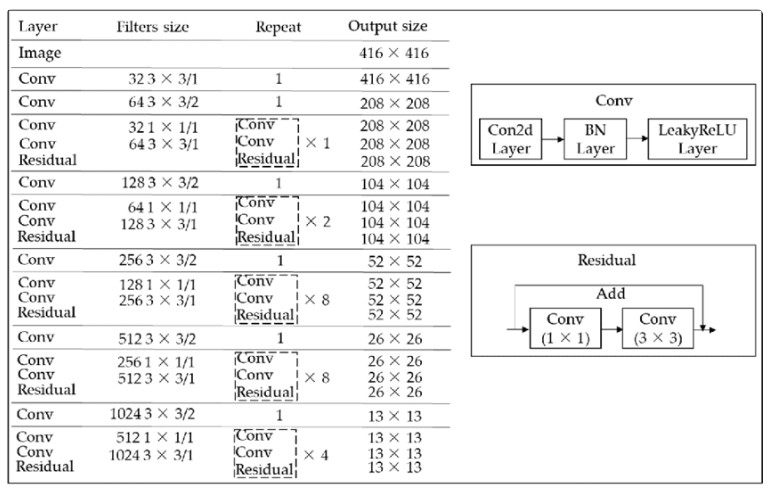
\includegraphics[scale=0.7]{gambar/diagramarsiyolov3.jpg}
  % Ubah dengan keterangan gambar yang diinginkan
  \caption{Diagram arsitektur YOLOv3}
  \label{fig:diagramyolov3}
\end{figure}

\subsubsection{Arsitektur YOLOv5}
\label{subsec:arsitektur-yolov5}
YOLOv5 memiliki perbedaan yang mencolok dibandingkan dengan versi YOLO sebelumnya. YOLOv5 memanfaatkan PyTorch alih-alih menggunakan
Darknet53 dan menggunakan CSPDarknet53 sebagai \emph{backbone}. \emph{Backbone} ini menyelesaikan pengulangan informasi gradien pada \emph{backbone} yang besar dan mengintegrasikan
perubahan gradien ke dalam \emph{feature map} yang dimana dapat mengurangi kecepatan inferensi, meningkatkan akurasi dan mengurangi ukuran model dengan cara mengurangi parameter. YOLOv5 menggunakan
\emph{path aggregation network}(PANet) sebagai \emph{neck} untuk meningkatkan alur penyampaian informasi. PANet mengadopsi \emph{feature pyramid network} (FPN) terbaru yang mencakup
beberapa lapisan \emph{bottom-up} dan \emph{top-down}. Hal ini meningkatkan propagasi pada \emph{low-level-feature} pada model. PANet meningkatkan lokalisasi pada \emph{lower-layers}, yang dimana meningkatkan akurasi
lokalisasi pada objek. Selain itu, \emph{head} pada YOLOv5 sama seperti YOLOv3 yang dimana menghasilkan tiga \emph{output} dari \emph{feature maps} untuk mendapatkan \emph{multi scale prediction}. 
Hal tersebut membantu meningkatkan prediksi objek kecil hingga objek besar secara efisien pada model. Gambar diumpankan kepada CSPDarknet53 untuk mengekstraksi fitur dan diumpankan lagi ke PANet untuk \emph{feature fusion}, 
pada akhirnya, lapisan YOLO dapat menghasilkan model. Arsitektur dari YOLOv5l dapat dilihat pada gambar 2.11, \emph{focus layer} pada YOLOv5 merupakan pengembangan dari arsitektur YOLOv3 dengan cara menggantikan tiga \emph{layer}
pertama pada YOLOv3 dan membuar sebuah \emph{layer} tunggal pada YOLOv5. Selain itu pada YOLOv5 \emph{Conv} menunjukkan \emph{convolution-layer}. C3 terdiri dari tiga \emph{convolution-layers} dan sebuah modul yang berjalan dengan berbagai
hambatan. \emph{Spatial Pyramid Pooling} (SPP) adalah penyatuan lapisan yang berguna untuk menghilangkan batasan ukuran \emph{network} yang tetap. \emph{Upsample} digunakan dalam tahap \emph{upsampling} pada \emph{layer fusion} sebelumnya pada
\emph{node} terdekat. \emph{Concat} merupakan \emph{slicing layer} yang digunakan memotong lapisan sebelumnya. Terakhir adalah Conv2d yang merupakan modul deteksi yang digunakan sebagai \emph{head} dari jaringan.
Perbedaan yang paling utama pada YOLOv5 ini adalah diperkenalkannya \emph{focus layer}. \emph{Focus layer} menggantikan tiga \emph{layer} pertama pada YOLOv3, keunggulan dari \emph{focus layer} ini adalah mengurangi penggunaan memori CUDA, mengurangi
\emph{layer}, dan \emph{forward propagation} dan \emph{back propagation} yang meningkat.

\begin{figure}[ht]
  \centering
  % Ubah dengan nama file gambar dan ukuran yang akan digunakan
  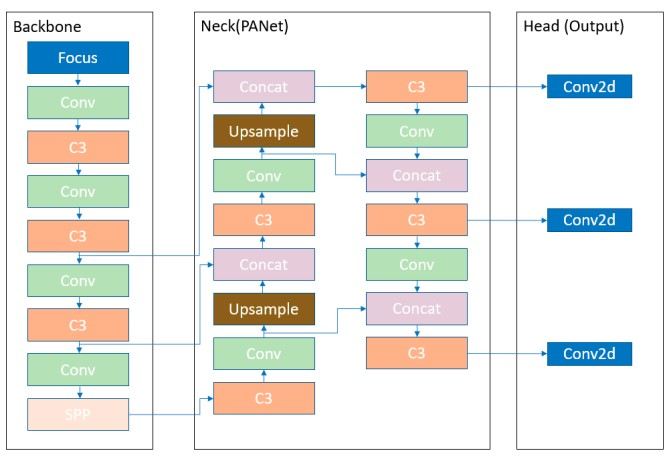
\includegraphics[scale=0.8]{gambar/arsitektur_yolov5.jpg}
  % Ubah dengan keterangan gambar yang diinginkan
  \caption{Diagram arsitektur YOLOv5}
  \label{fig:diagramyolov5}
\end{figure}

\subsection{Metode Pengujian}
\label{sec:metode-pengujian}

\subsubsection{\emph{Confusion Matrix}}
\label{subsec:confusion-matrix}

\emph{Confusion matrix} merupakan tabel yang digunakan untuk menggambarkan kinerja dari \emph{classifier} dengan beberapa data uji
yang sudah diketahui nilainya. Sehingga menciptakan sebuah visualisasi bagaimana kinerja pada suatu algoritma dan mengidentifikasi
\emph{confusion} antar kelas seperti kesalahan pemberian label oleh prediksi model. Contoh
dari \emph{confusion matrix} dapat dilihat pada tabel 2.2.

\emph{Confusion matrix} adalah sebuah ringkasan hasil dari prediksi dalam permasalahan klasifikasi,
Jumlah prediksi yang benar dan salah
dikumpulkan dengan nilai-nilai hitung dan dipecah oleh masing - masing
kelas. Sehingga dengan Confusion Matrix tidak hanya memberikan
informasi kesalahan yang dibuat \emph{classifier} tetapi juga jenis
kesalahannya. Pada \emph{confusion matrix}, terdapat beberapa ketentuan sebagai berikut:
\begin{table}[]
  \caption{Contoh dari \emph{confusion matrix}}
  \centering
  \begin{tabular}{ll|cc|}
  \cline{3-4}
                                                  &                              & \multicolumn{2}{c|}{Kondisi Aktual}    \\ \cline{3-4} 
                                                  &                              & \multicolumn{1}{c|}{Positif} & Negatif \\ \hline
  \multicolumn{1}{|c|}{\multirow{2}{*}{Prediksi}} & \multicolumn{1}{c|}{Positif} & \multicolumn{1}{c|}{TP}      & FP      \\ \cline{2-4} 
  \multicolumn{1}{|c|}{}                          & \multicolumn{1}{c|}{Negatif} & \multicolumn{1}{c|}{FN}      & TN      \\ \hline
  \end{tabular}
\end{table}
\begin{enumerate}
  \item \emph{Positive} (P): Kondisi aktual bernilai positif.
  \item \emph{Negative} (N): Kondisi aktual bernilai negatif.
  \item \emph{True Positive} (TP): Kondisi aktual bernilai positif, dan nilai prediksi positif.
  \item \emph{True Negative} (TN): Kondisi aktual bernilai positif, dan nilai prediksi negatif.
  \item \emph{False Positive} (FP): Kondisi aktual bernilai negatif, dan nilai prediksi negatif.
  \item \emph{False Negative} (FN): Kondisi aktual bernilai negatif, dan nilai prediksi bernilai positif.
\end{enumerate}

\subsubsection{\emph{Recall}}
\label{subsec:recall}

\emph{Recall} dapat diartikan sebagai rasio dari total jumlah kondisi aktual bernilai positif dan nilai prediksi positif (\emph{True Positive}) dibandingkan
dengan jumlah total contoh positif. \emph{High recall} menunjukkan bahwa sebuah kelas dikenali dengan benar (FN sedikit). \emph{Recall} dapat dihitung menggunakan 
persamaan 2.5.

\begin{equation}
  Recall = \frac{TP}{TP + FN}
\end{equation}

\subsection{\emph{Precision}}
\label{subsec:precision}

Nilai \emph{precision} merupakan nilai yang didapatkan dari jumlah kondisi aktual bernilai positif yang diklasifikasikan dengan benar berbanding dengan kondisi Aktual
positif yang diklasifikasikan dengan benar dan dijumlahkan dengan kondisi aktual positif yang diklasifikan dengan salah. Nilai \emph{Precision} tinggi menunjukkan
contoh berlabel positif dan klasifikasi positif (FP sedikit), untuk rumusnya dapat dilihat sebagai berikut.

\begin{equation}
  Precision = \frac{TP}{TP + FP}
\end{equation}

\begin{enumerate}
  \item \emph{High Recall, Low Precision}: menandakan sebagian besar contoh positif dapat dikenali dengan benar (nilai FN rendah) akan tetapi ada banyak positif palsu
  \item \emph{Low Recall, High Precision}: menandakan model kehilangan banyak contoh positif (FN tinggi) tetapi yang diprediksi positif benar positif (FP Rendah)
\end{enumerate}

\subsubsection{\emph{F-Measure}}
\label{subsec:f1-score}

\emph{F-Measure} atau dikenal juga sebagai \emph{F1 Score} merupakan perbandingan dari rata - rata nilai \emph{Precision} dan \emph{Recall} yang dibobotkan seperti persamaan 2.7 berikut.
\begin{equation}
  FMeasure = \frac{2 \times recall \times precision}{Recall + Precision}
\end{equation}

\subsubsection{\emph{Intersection over Union} (IoU)}
\label{subsec:IoU}
\emph{Intersection over Union} merupakan sebuah metrik evaluasi untuk mengukur keakuratan detektor objek pada \emph{dataset} tertentu. IoU dapat
digunakan dengan ketentuan sebagai berikut:
\begin{enumerate}
  \item Memiliki \emph{ground-truth box} pada \emph{dataset} objek
  \item Prediksi \emph{bounding-box} pada dataset objek
\end{enumerate}
Ilustrasi perbandingan \emph{ground-truth bounding box} dan \emph{predicted bounding box} dari model seperti Gambar 2.12. \emph{Intersection over Union} (IoU) merupakan perbandingan
antara \emph{ground-truth bounding box} dengan \emph{predicted bounding box} pada model sesuai dengan persamaan 2.8. Persamaan tersebut dapat diilustrasikan seperti pada Gambar 2.13.
\begin{equation}
  IoU = \frac{A \bigcap B}{A \bigcup B}
\end{equation} 

\begin{figure}[ht]
  \centering
  % Ubah dengan nama file gambar dan ukuran yang akan digunakan
  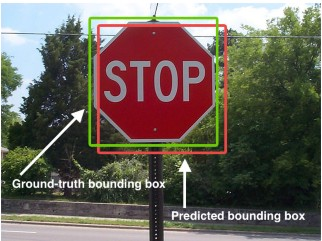
\includegraphics[scale=1]{gambar/ilustrasi-iou.jpg}
  % Ubah dengan keterangan gambar yang diinginkan
  \caption{Ilustrasi \emph{Predicted} dan \emph{Ground-truth bounding box} pada \emph{Intersection over Union}}
  \label{fig:gambar-iou}
\end{figure}

\begin{figure}[ht]
  \centering
  % Ubah dengan nama file gambar dan ukuran yang akan digunakan
  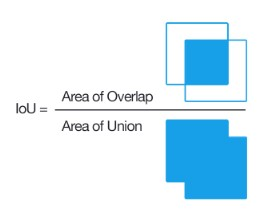
\includegraphics[scale=0.8]{gambar/ilustrasi-iou-rumus.jpg}
  % Ubah dengan keterangan gambar yang diinginkan
  \caption{Ilustrasi Persamaan \emph{Intersection over Union}}
  \label{fig:gambar-iou-rumus}
\end{figure}

\subsubsection{\emph{mean Average Precision} (mAP)}
\label{subsec:mAP}

\emph{mean Average Precision} (mAP) merupakan nilai rata-rata dari \emph{Average Precision} (AP) yang membentuk sebuah metrik evaluasi
untuk mengukur kinerja dari sebuah deteksi objek. Nilai AP didapatkan dari perhitungan \emph{precision} pada persamaan 2.6 dan perhitungan
\emph{recall} pada persamaan 2.5 yang selanjutnya dilakukan perhitungan seperti pada persamaan 2.9 dan 2.10 berikut.
\begin{equation}
  AP = \sum (recall_{n+1}-recall_{n}) \times precision_{interp} \times (recall_{n+1})
\end{equation}
\begin{equation}
  p_{interp}(r_{n+1}) = \underset{r\geq r_{n+1}}{max} p(\tilde{r})
\end{equation}
